% To build everything run
%	latexmk -xelatex
% To clean temporary files run
%	latexmk -c
\documentclass[12pt]{scrreprt}

% German locale
\usepackage[T1]{fontenc}
\usepackage[ngerman]{babel}

% Use APA citation
%\usepackage[natbibapa]{apacite}
\usepackage{csquotes}
\usepackage[backend=biber, style=apa, autocite=footnote]{biblatex}
	\bibliography{example}

% Add images
\usepackage{graphicx}

% Blind text
\usepackage{lipsum}

% Configure fonts
% Comment out when fonts are not found or use different fonts
%\usepackage{lmodern}
\usepackage{fontspec}
	\setmainfont{TeX Gyre Pagella}
	\setsansfont{TeX Gyre Heros}

% Define layout
\usepackage{setspace}
	\setstretch{1.41}
\usepackage[
	a4paper,
	left		= 2.5cm,
	right		= 3cm,
	top			= 2cm,
	bottom	= 2cm,
	%includeheadfoot,
	%showframe
	]{geometry}

\usepackage{scrlayer-scrpage}
\usepackage[bottom]{footmisc}
	\clearpairofpagestyles

	\setkomafont{pageheadfoot}{\rmfamily}
	%\setkomafont{pagehead}{\bfseries}
	\setkomafont{pagination}{}

	\KOMAoptions{
	   headsepline = true,
	   footsepline = false,
	   %plainfootsepline = true,
	}

	\automark[chapter]{chapter}

	\ihead{\headmark}
	\ohead{\pagemark}

\title{Das linguistische Relativitätsprinzip}
\author{Jasper Gude}
\date{\today{}, Hockenheim}

\begin{document}

\maketitle

\begin{center}
	\bfseries{Eigenständigkeitserklärung}
\end{center}
Ich versichere, dass ich diese Ausarbeitung selbständig verfasst, alle aus anderen Werken
wörtlich oder sinngemäß entnommenen Stellen unter Angabe der Quelle als Entlehnung
kenntlich gemacht und andere als die angegebenen Hilfsmittel nicht benutzt habe.

Oftersheim, \today, Unterschrift

\tableofcontents
\listoffigures
\listoftables

\chapter{Kapitelüberschrift}
	\label{chap:kapitel}

\section{Abschnittüberschrift}
	\label{sec:abschnitt}
\lipsum[2-4]
\autocite[5]{a}

\subsection{Unterabschnittüberschrift}
	\label{sec:unterabschnitt}
\lipsum[1-2]
\autocite[1--5]{b}

\begin{figure}[!htb]
	\centering
	  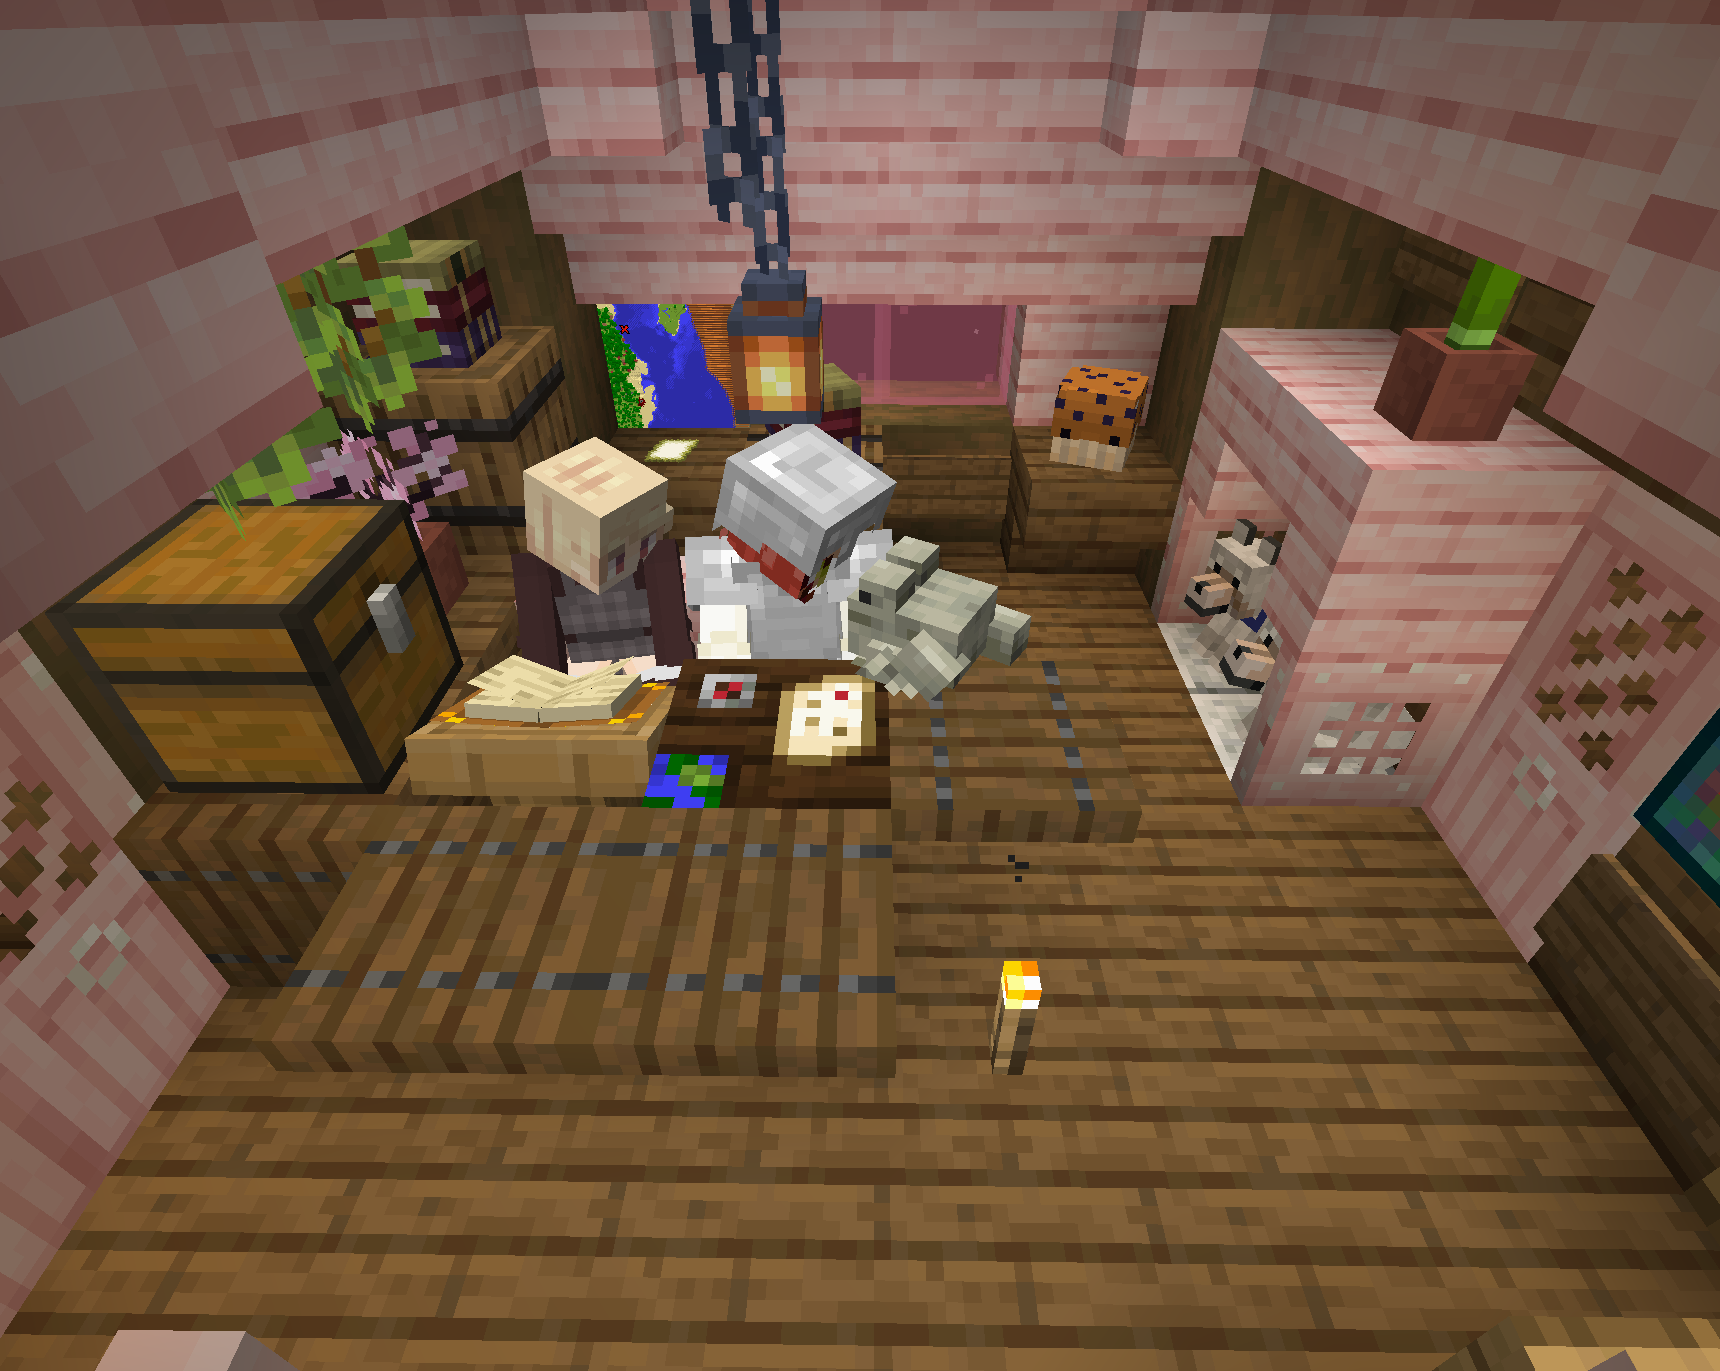
\includegraphics[width=0.5\textwidth]{image}
	\caption{Stare-off with grandma}
	\label{fig:granny}
\end{figure}

\subsubsection{Unterunterabschnittüberschrift}
	\label{sec:unterunterabschnitt}
\lipsum[1-1]
\autocite[30--58]{c}

\printbibliography

\end{document}
